


The model might be expected to start in the same way as Peierls; bringing together two half crystals as shown in \autoref{fig:semi_infinite_crystals} and simply allowing the structure to relax, leaving all the atomic positions as free variables. However there are two reasons to apply constraints to the atomic coordinates. Firstly constraints reduce the number of parameters to search. Secondly an unconstrained global optimiser might remove the dislocation entirely to create a perfect crystal, since dislocations are not equilibrium defects the most stable configurations for the atoms would be in a defect free crystal. To achieve this a displacement field based on initial atomic coordinates is used to find a final atomic configuration.

For a given value of $\alpha$ there will be an initial configuration of atoms defined by two half crystals brought together at a slip plane with some relative displacement between them defined by $\alpha$ and the Burgers vector. The core of the dislocation is taken to be the line where $x,y = 0$. The position of the core with respect to the lattice of the half crystals is defined by $\alpha$, usually with $\alpha=0$ defining the configuration in which the extra half-plane of atoms aligns with the dislocation core, as shown in \autoref{fig:joined_half_crystals}. 

The final, in the sense of ready to be evaluated energetically rather than optimised, configuration is the combination of  the initial positions and an array of displacements defined by some displacement field, $\bm{\delta}(x_0, y_0, z_0)$, i.e.
\begin{equation}
\mathbf{r}_i = \mathbf{r}_i^0 + \bm{\delta}(\bm{r}_i^0)
\end{equation}
where $\mathbf{r}_i$ is the position vector defining the final position of the $i$th atom, $\mathbf{r}_i^0$ is the vector defining the initial position of the $i$th ion and $\bm{\delta}$ is a vector displacement field.


%%%%%%%%%%%%%%%%%%%%%%%%%%%%%%%%%%%%%%%%%%%%%%%%%%%%%%%%%%%%%%%%%%%%%%%%%%%5
%
%                      Initial half crystals
%
%%%%%%%%%%%%%%%%%%%%%%%%%%%%%%%%%%%%%%%%%%%%%%%%%%%%%%%%%%%%%%%%%%%%%%%%%%%%%%
\subsection{Defining the initial atomic positions}


Firstly we must define the initial positions of the atoms in the half crystals. In the Peierls model the material was assumed to be a simple orthorhombic lattice; i.e. a misaligned  bond across the slip plane has a minimum energy when the bond is normal to the slip plane. To consider the effects of the particular structure the atomic configuration must be generated from the lattice and motif of the perfect crystal.

To create a crystal conveniently oriented with respect to the Cartesian reference axes and the crystal slip system unconventional unit cells were defined. Directions and planes defined relative to the unconventional or dislocation cell will be marked prime, e.g. $[1\,0\,0]'$. The Burgers vector $\mathbf{b}$ is taken to be the $[1\,0\,0]'$, the shortest slip plane normal that is a full lattice vector is taken to be $[0\,1\,0]'$ and the $[0\,0\,1]'$, parallel to the line vector, is the shortest lattice vector that is perpendicular to both the Burgers vector and the slip plane normal and its sign is such that the axes are right handed. Filling space by combining a motif and a lattice defined according to these axes is convenient because most of the mathematical results of dislocation theory, stress and strains fields etc., are defined taking $x$, $y$ and $z$ parallel to $[1\,0\,0]'$, $[0\,1\,0]'$, $[0\,0\,1]'$ respectively.

For example the \ce{NaCl} <1\,\={1}\,0>\{1\,1\,0\} slip system gives a new unit cell aligned with the slip system:

\begin{equation*}
\begin{aligned}[c]
{[1\,0\,0]}' &=\, ^{1}\!/_{2} [1\,1\,0]   \\
{[0\,1\,0]}' &=\, ^{1}\!/_{2} [1\,\overline{1}\,0]   \\
{[0\,0\,1]}' &=\, [0\,0\,1]   
\end{aligned}[c]
\qquad
\begin{aligned}[c]
&\parallel \mathbf{b} \\
&\parallel \mathbf{d} \\
&\parallel \mathbf{l}
\end{aligned}
\end{equation*}
where $\mathbf{l}$ is the line vector of the dislocation.


The atoms in this non-conventional unit cell are
$$
motif = \begin{pmatrix}
0 & 0 & 0 & +1 \\
^{1}\!/_{2} & ^{1}\!/_{2} & ^{1}\!/_{2} & +1 \\
0 & 0 & ^{1}\!/_{2} & -1 \\
^{1}\!/_{2} & ^{1}\!/_{2} & 0 & -1 \\
\end{pmatrix}
$$
where a $+1$ in the final column denotes the positive charge of a sodium ion and a $-1$ denotes the negative charge of a chloride ion.



\begin{figure}
\centering


    \begin{subfigure}{0.55\textwidth}
    \centering
    \includegraphics[width=\textwidth]{NaCl_conventional_unit_cell}
    \caption{The conventional unit cell of sodium chloride with the salient slip directions and plane normals highlighted. \label{fig:NaCl_conventional_cell_slip_system_marked}}
    \end{subfigure}

    \begin{subfigure}{0.4\textwidth}
    \centering
    \includegraphics[height=2.0in]{NaCl_110_110}
    \caption{The sodium chloride unit cell best aligned with the <1\,1\,0>\{1\,\={1}\,0\} slip system. \label{fig:NaCl_110_110_unit_cell}}
    \end{subfigure}
    ~
    \begin{subfigure}{0.4\textwidth}
    \centering
    \includegraphics[height=2.5in]{NaCl_110_001}
    \caption{The sodium chloride unit cell best aligned with the <1\,1\,0>\{0\,0\,1\} slip system. \label{fig:NaCl_110_001_unit_cell}}
    \end{subfigure}

\caption[Unconventional unit cells of rock salt to build a dislocation.]{Possible unit cells for sodium chloride showing the conventional unit cell and two unconventional unit cells with the new crystallographic axes aligned to slip system, i.e. the Burgers vector and slip plane normal.\label{fig:unconventional_NaCl_unit_cells}}
\end{figure}






Similarly the \ce{NaCl} <1\,\={1}\,0>\{0\,0\,1\} slip system is defined by the unit cell:
\begin{equation*}
\begin{aligned}[c]
 {[1\,0\,0]}' &=\, ^{1}\!/_{2} [1\,1\,0] \\
 {[0\,1\,0]}' &=\,  [0\,0\,1] \\
 {[0\,0\,1]}' &=\; ^{1}\!/_{2} [1\,\overline{1}\,0] \\
\end{aligned}
\qquad
\begin{aligned}[c]
&\parallel \mathbf{b} \\
&\parallel \mathbf{d} \\
&\parallel \mathbf{l}
\end{aligned}
\end{equation*}
and the atoms are
$$
motif = \begin{pmatrix}
0 & 0 & 0 & +1 \\
^{1}\!/_{2} & ^{1}\!/_{2} & ^{1}\!/_{2} & +1 \\
^{1}\!/_{2} & 0 & ^{1}\!/_{2} & -1 \\
0 & ^{1}\!/_{2} & 0 & -1
\end{pmatrix}
$$


These unit cells are shown in relation to the conventional cell in \autoref{fig:unconventional_NaCl_unit_cells}. With these unit cells we can convolve the motif with a lattice to generate an initially perfect crystal defined with respect to Cartesian axes aligned with the slip system. Two offsets are then applied; firstly the half crystal below the slip plane, which is defined by $y < 0$, will be offset in the positive $x$ direction by $b/2$ and then the entire crystal is offset to put the dislocation core in the desired location. The latter will require an offset along the slip direction, $[0\,0\,1]'$ of $\alpha b$ and an additional offset in the $[0\,1\,0]'$ direction. While the magnitude of this offset is not necessarily predictable in the case of \ce{NaCl} the core must be at a height of $d/4$ in order to be halfway between the two (0\,2\,0) layers.

So the initial positions of the atoms in the dislocated crystal are related to those of an initially perfect crystal by
\begin{equation}
\bm{r_i^0} = \bm{r_i^{\text{perfect}}} +\begin{cases}
[-\alpha{}b, h, 0] & \quad \text{if } y_i^{\text{perfect}} > 0\\
[b(1/2 - \alpha{}), h, 0] & \quad \text{if } y_i^{\text{perfect}} < 0\\
\end{cases} 
\end{equation}

The offset to the atomic coordinates in $-\alpha{}b$ such that as $\alpha$ increases the dislocation motion is in the positive $x$ direction.





\FloatBarrier












%%%%%%%%%%%%%%%%%%%%%%%%%%%%%%%%%%%%%%%%%%%%%%%%%%%%%%%%%%%%%%%%%%%%%%%%%%%%%%%%%%%

                          % Displacement fields

\subsection{Displacement fields}

A suitable displacement field is required. First we can take a Volterra dislocation, which in a continuous isotropic elastic medium has a displacement field \cite{hirth_lothe1982volterra_displacements}:
\begin{subequations}
\begin{align}
u^x &= \frac{b}{2\pi}\left[ \arctan\left(\frac{x}{y}\right) + \frac{xy}{2(1-\nu)(x^2 + y^2)} \right] \\[0.5ex]
v^y &= -\frac{b}{2\pi} \left[ \frac{1-2\nu}{4(1-\nu)} \ln(x^2 + y^2) + \frac{x^2 + y^2}{4(1-\nu)(x^2 + y^2)} \right]
\end{align}
\end{subequations}
where $u^x$ and $v^y$ are the components of the displacement field parallel to $x$ and $y$ respectively, $x$ is the initial position parallel to the Burgers vector, $y$ is the initial position parallel to the slip plane normal, $b$ is the magnitude of the Burgers vector and $\nu$ is the Poisson ratio of the material. The terms all converge to fixed values at large $x$ or $y$ except the logarithmic component of $v^y$. This represents the bending of a single crystal that arises from the introduction of an extra half plane \cite{hirth_lothe1982volterra_displacements}.

This formulation of the displacement field and subsequent solution for an isotropic elastic continuum is discontinuous, diverging at $r=0$, where $r=\sqrt[]{x^2+y^2}$. To remove the discontinuity \citet{Eshelby1949} proposed considering a single dislocation to be composed of a continuous distribution of dislocations with infinitesimal Burgers vectors, the integral of which yields the Burgers vector of the full dislocation. 

By considering the local strains (a normal strain parallel to the slip plane) due to this distribution and integrating the stress on the slip plane can be found. By applying a force balance condition with the misalignment term the displacements at the slip plane can be found:


If $\bm{b}'(x')\mathrm{d}x'$ is the Burgers vector of an infinitesimal dislocation between $x'$ and $x'+\mathrm{d} x'$, and displacements in $y$ are assumed to be small, this can be related to the displacement, $u^x$, since the local displacement will be given by $-2(\mathrm{d} u^x/\mathrm{d} x)\mathrm{d} x'$ \cite{hirth_lothe1982peierls_displacements} we can write


\begin{equation}
b = \int_{-\infty}^{\infty} b'(x') \dd x' = -2\int^{\infty}_{-\infty} \left( \! \frac{\dd u^x}{\dd x} \right)_{x=x'} \dd x' 
\end{equation}
Using the result for a Volterra dislocation \cite{hirth_lothe_1982_volterra_stress_field}:
\begin{equation}
\sigma^{\text{Volterra}}_{xy} = \frac{\mu b}{2\pi (1-\nu)} \frac{x(x^2 - y^2)}{(x^2+y^2)^2}
\end{equation}
and setting $y=0$,
\begin{equation}
\sigma^{\text{volterra}}_{xy}(x,0) = -\frac{\mu}{2\pi(1-\nu)} \int^{\infty}_{-\infty} \frac{b'}{x-x'} \!\dd x' =  \frac{\mu}{\pi(1-\nu)} \int^{\infty}_{-\infty} \frac{1}{x-x'} \left(\!\frac{\dd u^x}{\dd x}\right)_{x=x'} \!\dd x'
\label{eqn:elastic_stress_at_slip_plane}
\end{equation}

At the minimum energy position the net stress at $(x,0)$ vanishes, so there must be a balancing stress arising from the misalignment of the material across the slip plane. By analogy with \citet{Frenkel1926}
\begin{equation}
\sigma_{xy}^{\text{misalignment}}(x,0) = C \sin \left( \frac{2\pi \phi^x}{b} \right)
\end{equation}
or in terms of the displacements either side of the slip plane:
\begin{equation}
\sigma_{xy}^{\text{misalignment}}(x,0) = -C \sin \left( \frac{4\pi u^x}{b} \right)
\end{equation}
If Hooke's law is satisfied at small strains we can write
\begin{equation}
\sigma_{xy}^{\text{misalignment}}(x,0) = 2 \mu \varepsilon_{xy} = \frac{\mu{}\phi^x}{d}
\label{eqn:misalign_stress_at_slip_plane}
\end{equation}
We can combine \autoref{eqn:elastic_stress_at_slip_plane} and \autoref{eqn:misalign_stress_at_slip_plane} to give a integral equation thus:
\begin{equation}
\int^{\infty}_{-\infty} \frac{1}{x-x'} \left(\!\frac{\dd u^x}{\dd x}\right)_{x=x'} \dd x' = \frac{b(1-\nu)}{2d} \sin\left(\frac{4\pi{}u^x}{b}\right)
\end{equation}
The solution is \cite{hirth_lothe1982peierls_displacements,Eshelby1949}
\begin{equation}
u^x(x) = -\frac{b}{2\pi} \arctan \left( \frac{x}{w} \right)
\label{eqn:one_dimensional_displacements}
\end{equation}
where $w$ is the half width of the dislocation and, for an isotropic elastic solid, has the value
\begin{equation}
w = \frac{d}{2(1-\nu)}.\label{eqn:half_width}
\end{equation}
\autoref{eqn:one_dimensional_displacements} satisfies the boundary condition that $u^x(\infty) = - u^x(-\infty) = -b/4$. Also $x=w$ gives $u^x(w)=1/2\, u^x(\infty)$, i.e. in the region $-w < x < w$ the disregistry across the slip plane is greater than half the maximum that occurs at $x=0$.

The two dimensional case gives a displacement field \cite{Eshelby1949,Leibfried1949,nabarro1987theory}:
\begin{subequations}\label{eqn:displacements}
\begin{align}
u^x(x,y) &= \frac{b}{2\pi} \left( \arctan \left[ \frac{y +  w\frac{|y|}{y}}{x} \right] - \frac{\pi}{2} \frac{|y|}{y} \frac{|x|}{x} \right) + c_1 \frac{xy}{x^{2} + (y + w\frac{|y|}{y} )^2} \\
v^y(x,y) &= c_2 \frac{y(y +  w \frac{|y|}{y})}{x^2 + (y +  w \frac{|y|}{y})^2} + c_3 \ln \left| \frac{x^2 + (y +  w \frac{|y|}{y})^2}{b^2} \right|
\end{align}
\label{eqn:displacement_field}
\end{subequations}
The final atomic configuration is then defined by 
\begin{equation}
\bm{r}_i = \bm{r}_i^0 + [u_i^x\,\bm{\mathrm{\hat{i}}},\; v_i^y\,\bm{\mathrm{\hat{j}}},\; 0\,\bm{\mathrm{\hat{k}}}]
\end{equation}

These terms can be interpeted physically; The arctan term is the same as in the original Peierls treatment, representing displacements along the slip plane that alter the local misalignment acorss the slip plane. The terms with the prefactors $c_1$ and $c_2$ represent shear strains, the $xy$ and $yx$ shears respectively. The logarithmic term, with the prefactor $c_3$, represents the bending of the entire crystal that must arise from the introduction of an extra halfplane of atoms. This logarithmic term does not converge to a constant value at large $x$ or $y$, but this is consistent with this physical interpretation \cite{hirth_lothe1982peierls_displacements}.

The inclusion of $v^y(x,y)$ in the displacement field means that there will always be some finite displacement normal to the slip plane. This is expected and will be associated with phenomena such as pressure dependent yield stress \cite{frost1982pressure}. These displacements might also be responsible for the normal strains observed around line defects in layered crystals that have been ascribed to ripplocations \cite{Gruber2016}.




For an isotropic elastic medium the various parameters in \ref{eqn:displacement_field} are analytically found to have fixed values for the lowest energy dislocation. The half-width, $w$, takes the same value as in \autoref{eqn:half_width} and the three other parameters are defined by
\begin{subequations}\label{eqn:disloc_params}
\begin{align}
c_1 &= \frac{b}{4\pi{}(1-\nu)} \\
c_2 &= \frac{b}{4\pi{}(1-\nu)} \\
c_3 &= - \frac{b(1-2\nu)}{8\pi(1-\nu)}.
\end{align}
\label{eqn:expressions_for_the_ideal_disloca_parameters}
\end{subequations}
The terms of the form $|x|/x$ and $|y|/y$ are to give all the terms the right sense in the right regions of space, i.e. above and below the slip plane in $y$ and either side of the dislocation in $x$. This reduces to the simpler solution in \autoref{eqn:one_dimensional_displacements} if only the atoms adjacent to the slip plane are considered. This form is useful because it is continuous and finite for all values of $x$ and $y$. 


\begin{figure}
\centering

    \begin{subfigure}{0.4\textwidth}
    \centering
    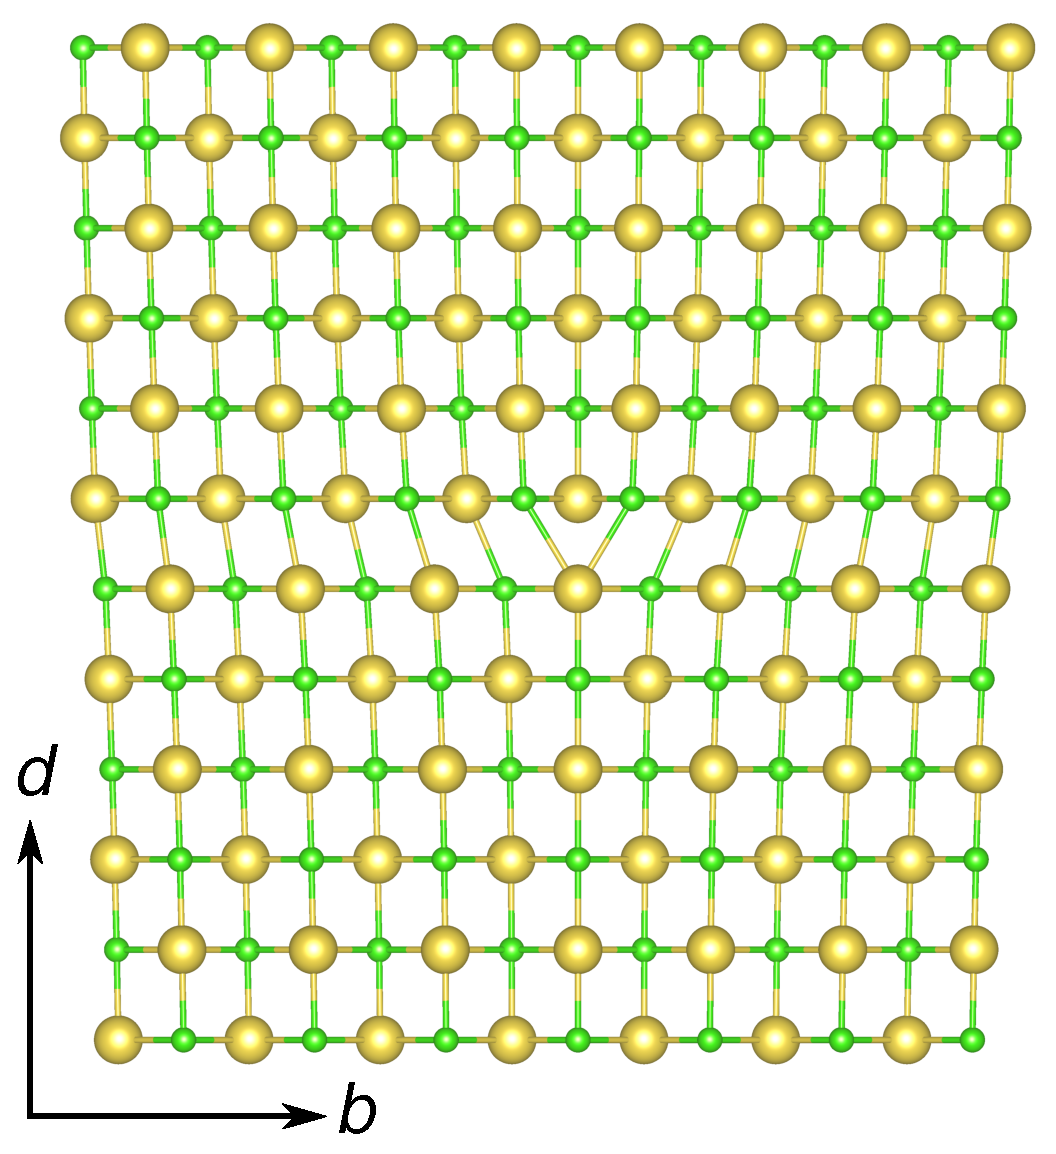
\includegraphics[width=0.6\textwidth]{wide_NaCl}
    \caption{A dislocation with a large width.}
    \end{subfigure}
    ~
    \begin{subfigure}{0.4\textwidth}
    \centering
    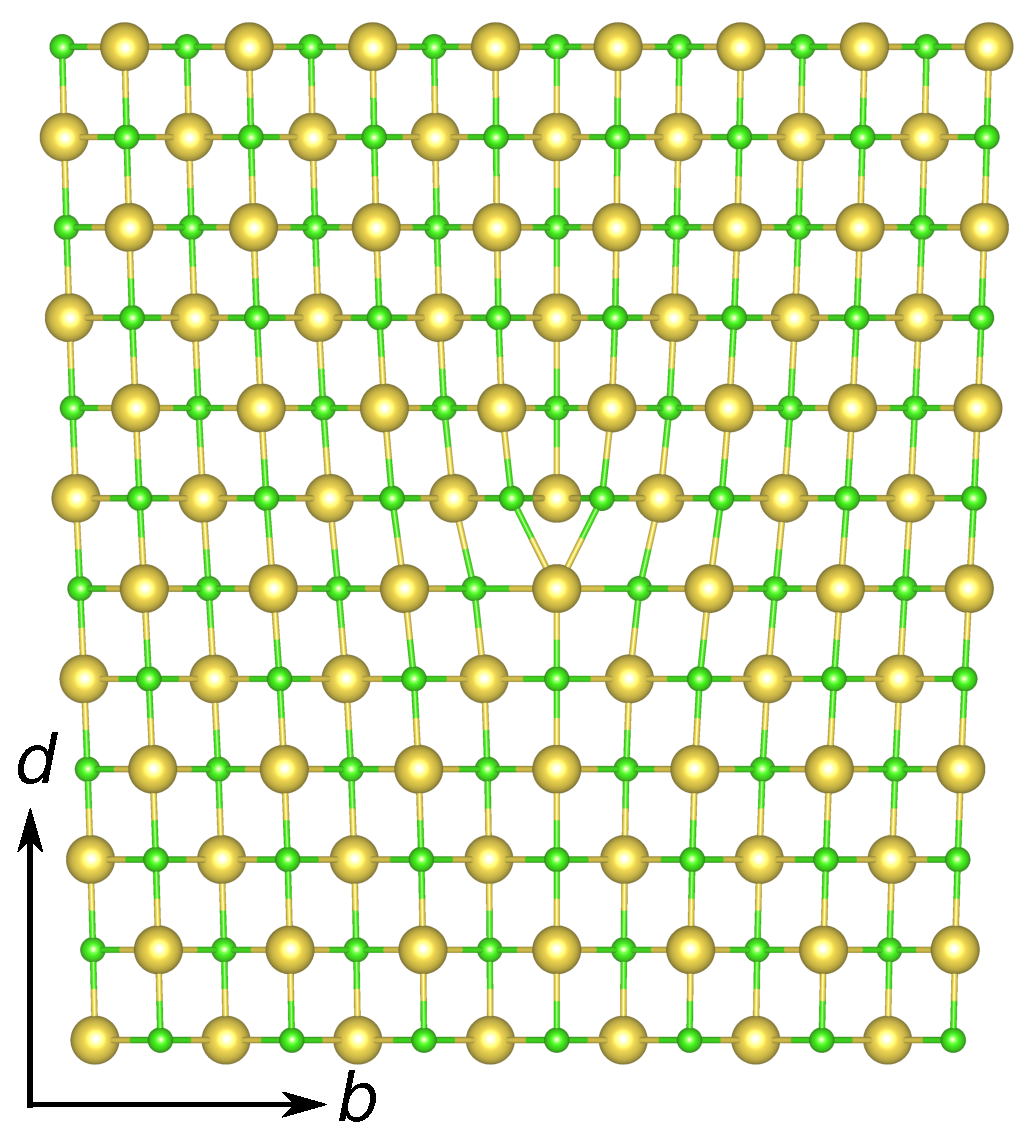
\includegraphics[width=0.6\textwidth]{narrow_NaCl}
    \caption{A dislocation with a small width.}
    \end{subfigure}

	\begin{subfigure}{0.4\textwidth}
	\centering
    \includegraphics[width=0.6\textwidth]{large_c1_NaCl}
    \caption{Large values of $c_1$ and $c_2$.}
	\end{subfigure}
    ~
	\begin{subfigure}{0.4\textwidth}
	\centering
    \includegraphics[width=0.6\textwidth]{large_c3_NaCl}
    \caption{A large value of $c_3$.}
	\end{subfigure}

    \begin{subfigure}{0.8\textwidth}
    \centering
    \includegraphics[width=0.5\textwidth]{typical_NaCl}
    \caption{A ``typical'' configuration.}
    \end{subfigure}

\captionsetup{width=0.8\textwidth}
\caption[The displacement field around an edge dislocation in rock salt.]{Various configurations of sodium chloride <1\,1\,0>\{0\,0\,1\} dislocations demonstrating the effects of the parameters of the displacement field defined in \autoref{eqn:displacements}, $w$, $c_1$, $c_2$ and $c_3$. Typical parameters are taken to be those predicted for an isotropic elastic material as given in  Equations~\ref{eqn:half_width} and \ref{eqn:disloc_params}, giving \SI{1.78}{\angstrom}, \SI{0.40}{\angstrom}, \SI{0.40}{\angstrom} and \SI{-0.12}{\angstrom} respectively for sodium chloride. Exaggerated values were ten times that. Calculated with $\nu =$~\num{0.207} and $a =$~\SI{5.644}{\angstrom} \cite{Theocaris1994,Rao1990}.\label{fig:parameters_of_the_disloc_configuration}}
\end{figure}


This gives a displacement field for a general material in which has four parameters; the width, $w$, and the scaling factors, $c_1$, $c_2$ and $c_3$. These parameters are varied to find the lowest energy dislocation. If the energy is calculated by an atomistic model, rather than by continuum elasticity, then there is no analytical solution for these parameters. Instead those values that minimise the energy are taken to be the correct solution.

The width of the dislocation still defines the region with large disregistries, while $c_1$ and $c_2$ define the magnitude of displacements associated with shear strains around the dislocation core and $c_3$ defines the magnitude of the bending of a crystal that must arise from the introduction of an extra half plane.
To illustrate the displacements produced by these different terms some exaggerated dislocation configurations are shown in \autoref{fig:parameters_of_the_disloc_configuration}.





A final note on the parametrisation of the dislocation structure is that the values $c_1$, $c_2$ and $c_3$ are not constrained. The purely isotropic case described above the parameters $c_1$, $c_2$ are positive and $c_3$ is negative, but there is no physical reason they cannot have a different sign. However a negative value of the width is not meaningful in this formulation. A negative width reintroduces the discontinuity at which displacements would diverge (in fact it would introduce two, one either side of the slip plane) which cannot be actually exist. Hence the constraint that $w>0$ is applied, but $c_1$, $c_2$ and $c_3$ are allowed to vary freely.




























